\documentclass[10pt]{article}

\usepackage[a4paper,margin=19mm]{geometry}
\usepackage{amsmath,amssymb}
\usepackage{caption}
\usepackage{subcaption}
\usepackage{microtype}
\usepackage{pgfplots}
\usepackage{tikz}

\pgfplotsset{compat=1.18}
\usetikzlibrary{calc}

\definecolor{rainfour}{RGB}{203,226,240}
\definecolor{rainfourmid}{RGB}{142,193,220}
\definecolor{rainfourhalf}{RGB}{105,169,207}
\definecolor{rainfive}{RGB}{49,121,179}
\definecolor{linkblue}{RGB}{0,76,153}
\definecolor{auxlink}{RGB}{80,80,80}

\newcommand{\raincell}[4]{%
  \path[fill=#4] (#1,#2) rectangle ++(1,1);
  \draw[black!75,line width=0.45pt] (#1,#2) rectangle ++(1,1);
  % Keep the numerical label above the link so both remain legible.
  \node[font=\small] at (#1+0.5,#2+0.72) {#3};
}

\newcommand{\truthfield}{%
  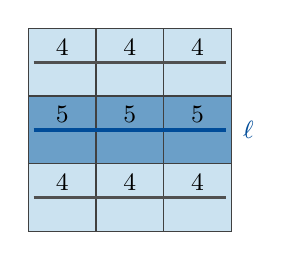
\begin{tikzpicture}[x=0.86cm,y=0.86cm]
    \raincell{0}{2}{$4$}{rainfour}
    \raincell{1}{2}{$4$}{rainfour}
    \raincell{2}{2}{$4$}{rainfour}
    \raincell{0}{1}{$5$}{rainfive!72}
    \raincell{1}{1}{$5$}{rainfive!72}
    \raincell{2}{1}{$5$}{rainfive!72}
    \raincell{0}{0}{$4$}{rainfour}
    \raincell{1}{0}{$4$}{rainfour}
    \raincell{2}{0}{$4$}{rainfour}
    \draw[auxlink,line width=1.0pt] (0.08,2.5) -- (2.92,2.5);
    \draw[linkblue,line width=1.7pt] (0.08,1.5) -- (2.92,1.5)
      node[right=2pt,font=\small,text=linkblue] {$\ell$};
    \draw[auxlink,line width=1.0pt] (0.08,0.5) -- (2.92,0.5);
  \end{tikzpicture}%
}

\newcommand{\idwfield}{%
  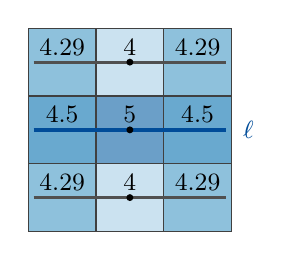
\begin{tikzpicture}[x=0.86cm,y=0.86cm]
    \raincell{0}{2}{$4.29$}{rainfourmid}
    \raincell{1}{2}{$4$}{rainfour}
    \raincell{2}{2}{$4.29$}{rainfourmid}
    \raincell{0}{1}{$4.5$}{rainfourhalf}
    \raincell{1}{1}{$5$}{rainfive!72}
    \raincell{2}{1}{$4.5$}{rainfourhalf}
    \raincell{0}{0}{$4.29$}{rainfourmid}
    \raincell{1}{0}{$4$}{rainfour}
    \raincell{2}{0}{$4.29$}{rainfourmid}
    \draw[auxlink,line width=1.0pt] (0.08,2.5) -- (2.92,2.5);
    \draw[linkblue,line width=1.7pt] (0.08,1.5) -- (2.92,1.5)
      node[right=2pt,font=\small,text=linkblue] {$\ell$};
    \draw[auxlink,line width=1.0pt] (0.08,0.5) -- (2.92,0.5);
    \foreach \y in {0.5,1.5,2.5}
      \fill[black] (1.5,\y) circle[radius=1.25pt];
  \end{tikzpicture}%
}

\newcommand{\ildwfield}{%
  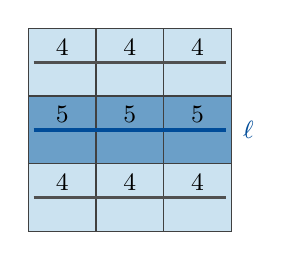
\begin{tikzpicture}[x=0.86cm,y=0.86cm]
    \raincell{0}{2}{$4$}{rainfour}
    \raincell{1}{2}{$4$}{rainfour}
    \raincell{2}{2}{$4$}{rainfour}
    \raincell{0}{1}{$5$}{rainfive!72}
    \raincell{1}{1}{$5$}{rainfive!72}
    \raincell{2}{1}{$5$}{rainfive!72}
    \raincell{0}{0}{$4$}{rainfour}
    \raincell{1}{0}{$4$}{rainfour}
    \raincell{2}{0}{$4$}{rainfour}
    \draw[auxlink,line width=1.0pt] (0.08,2.5) -- (2.92,2.5);
    \draw[linkblue,line width=1.7pt] (0.08,1.5) -- (2.92,1.5)
      node[right=2pt,font=\small,text=linkblue] {$\ell$};
    \draw[auxlink,line width=1.0pt] (0.08,0.5) -- (2.92,0.5);
  \end{tikzpicture}%
}

\newcommand{\profileplot}[3]{%
  \begin{tikzpicture}
    \begin{axis}[
      width=0.98\linewidth,
      height=3.55cm,
      xmin=0.72,xmax=3.28,
      ymin=3.8,ymax=5.2,
      xtick={1,2,3},
      xticklabels={1st pixel,2nd pixel,3rd pixel},
      ytick={4,4.5,5},
      xlabel={pixel crossed by $\ell$ (left to right)},
      ylabel={rain rate (mm/h)},
      tick label style={font=\scriptsize},
      label style={font=\scriptsize},
      grid=both,
      major grid style={black!15},
      axis line style={black!65},
      mark size=2.2pt,
    ]
      \addplot[linkblue,very thick,mark=*,mark options={fill=white}]
        coordinates {(1,#1) (2,#2) (3,#3)};
    \end{axis}
  \end{tikzpicture}%
}

\title{A $3\times3$ Illustration of Midpoint IDW and Link-Distance Weighting}
\author{}
\date{}

\begin{document}

\maketitle
\vspace{-2.5em}

\section{IDW Underestimate of Rain Rate}

We use a $3\times3$ field whose cell side length is $h$ and whose rain rates,
listed from top to bottom, are
\begin{equation}
R^{\mathrm{GT}}=
\begin{bmatrix}
4&4&4\\
5&5&5\\
4&4&4
\end{bmatrix}\ \mathrm{mm/h}.
\label{eq:gt-field}
\end{equation}
To obtain a valid example for the normalized IDW definition, place one
horizontal link through the center of each row.  The link-level rain rates are
then $4$, $5$, and $4$~mm/h, respectively.  We denote the middle link by
$\ell$ and examine the three pixels that it crosses.  All three links have
their midpoint in the middle column, and the IDW search radius is chosen larger
than $\sqrt{5}h$, so every link contributes at every non-midpoint cell.

For a pixel center $c_p$ that does not contain a link midpoint, midpoint IDW
with exponent two gives
\begin{equation}
\widehat R_p^{\mathrm{IDW}}
=
\frac{\displaystyle\sum_{j=1}^{3}
      \lVert c_p-m_j\rVert_2^{-2}R_j}
     {\displaystyle\sum_{j=1}^{3}
      \lVert c_p-m_j\rVert_2^{-2}},
\label{eq:idw}
\end{equation}
where $m_j$ and $R_j$ are the midpoint and rain rate of link $j$.  At the
center of the left or right pixel crossed by $\ell$, the distances to the
middle, upper, and lower link midpoints are $h$, $\sqrt{2}h$, and
$\sqrt{2}h$.  Therefore,
\begin{equation}
\widehat R_{1}^{\mathrm{IDW}}
=\widehat R_{3}^{\mathrm{IDW}}
=\frac{5h^{-2}+4(\sqrt{2}h)^{-2}+4(\sqrt{2}h)^{-2}}
       {h^{-2}+2(\sqrt{2}h)^{-2}}
=4.5\ \mathrm{mm/h}.
\label{eq:idw-crossed}
\end{equation}
The middle pixel contains the midpoint of $\ell$, so the discretized midpoint
rule sets its value directly to $R_\ell=5$~mm/h.  Repeating the same
calculation for the remaining cells gives
\begin{equation}
\widehat R^{\mathrm{IDW}}=
\begin{bmatrix}
73/17&4&73/17\\
9/2&5&9/2\\
73/17&4&73/17
\end{bmatrix}
\approx
\begin{bmatrix}
4.29&4&4.29\\
4.5&5&4.5\\
4.29&4&4.29
\end{bmatrix}\ \mathrm{mm/h}.
\label{eq:idw-field}
\end{equation}
Thus, along $\ell$, midpoint IDW underestimates the true rain rate in the two
off-center pixels, although it is exact in the midpoint pixel.

ILDW instead uses the distance from a pixel center to the full link segment
and applies the crossing-pixel rule.  If $C(p)$ denotes the set of links that
cross pixel $p$, then
\begin{equation}
\widehat R_p^{\mathrm{ILDW}}
=\frac{1}{|C(p)|}\sum_{j\in C(p)}R_j,
\qquad C(p)\ne\varnothing.
\label{eq:ildw-crossing}
\end{equation}
Every cell in a given row is crossed by that row's link.  Consequently ILDW
recovers the complete field in this example,
\begin{equation}
\widehat R^{\mathrm{ILDW}}=R^{\mathrm{GT}},
\end{equation}
and its profile along $\ell$ is uniformly $5$~mm/h.

\begin{figure}[p]
  \centering
  \begin{subfigure}[t]{0.38\textwidth}
    \centering
    \truthfield
    \caption{Ground-truth field and link geometry.}
  \end{subfigure}
  \hfill
  \begin{subfigure}[t]{0.57\textwidth}
    \centering
    \profileplot{5}{5}{5}
    \caption{Ground-truth profile along $\ell$.}
  \end{subfigure}

  \vspace{1.2em}

  \begin{subfigure}[t]{0.38\textwidth}
    \centering
    \idwfield
    \caption{Midpoint-IDW reconstruction. Dots mark the three virtual gauges.}
  \end{subfigure}
  \hfill
  \begin{subfigure}[t]{0.57\textwidth}
    \centering
    \profileplot{4.5}{5}{4.5}
    \caption{Midpoint-IDW profile along $\ell$.}
  \end{subfigure}

  \vspace{1.2em}

  \begin{subfigure}[t]{0.38\textwidth}
    \centering
    \ildwfield
    \caption{ILDW reconstruction.}
  \end{subfigure}
  \hfill
  \begin{subfigure}[t]{0.57\textwidth}
    \centering
    \profileplot{5}{5}{5}
    \caption{ILDW profile along $\ell$.}
  \end{subfigure}

  \caption{A concrete $3\times3$ example of the geometric difference between
  midpoint IDW and ILDW.  Midpoint IDW mixes the $5$~mm/h observation on the
  middle link with the two nearby $4$~mm/h observations away from the middle
  pixel, producing $(4.5,5,4.5)$~mm/h along $\ell$.  Since ILDW associates the
  link observation with every pixel crossed by its segment, it returns
  $(5,5,5)$~mm/h along $\ell$ and exactly reconstructs this row-wise-constant
  field.}
  \label{fig:idw-ildw-3x3}
\end{figure}

\paragraph{Why the literal single-link version does not work.}
If $\ell$ is the only link and $R_\ell=5$~mm/h, then for every in-radius
non-midpoint pixel the normalized IDW weight cancels:
\begin{equation}
\widehat R_p^{\mathrm{IDW}}
=\frac{\lVert c_p-m_\ell\rVert_2^{-2}R_\ell}
       {\lVert c_p-m_\ell\rVert_2^{-2}}
=R_\ell=5\ \mathrm{mm/h}.
\end{equation}
The midpoint rule gives the same value in the middle pixel.  Hence a setup
containing only one link cannot demonstrate IDW underestimation under the
normalized IDW definition; the two auxiliary links above are the minimal
addition that produces the intended comparison.  Alternatively, one would
have to replace normalized IDW by an unnormalized distance-decay kernel, which
would be a different estimator.

\end{document}
